\chapter{Экспериментальная часть}

\section{Замеры времени}

Благодаря распараллеливанию алгоритма обратной трассировки лучей
время работы было уменьшено.

Для замеров времени используется изображение размером 1200$\times$600.
Так как трассировка данного изображения считается достаточно короткой
задачей, используется усреднение времени, за которое проведён массовый эксперимент
(10 подходов).

Результат представлен на рис. \ref{ref:time}.

\begin{figure}[ht!]
	\centering{
		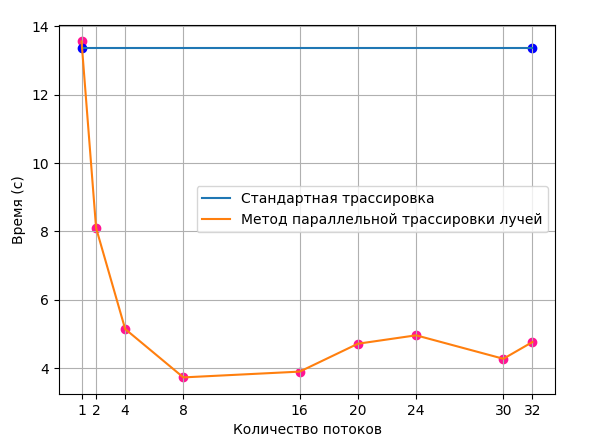
\includegraphics[width=0.7\textwidth]{time.png}
		\caption{Время работы последовательной и параллельной реализаций алгоритма трассировки}
		\label{ref:time}}
\end{figure}

\newpage

Последовательная реализация работает быстрее, чем создание одного потока,
потому что на создание потока тратится некоторое время.
При двух потоках выигрыш получается почти в два раза, так как два потока
трассируют одновременно свою часть экрана.
При увеличении числа потоков отслеживается уменьшение времени трассировки.
При 8 потоках достигается пик, при котором все ядра процессора одновременно
выполняют трассировку экрана.
Далее при увеличении числа потоков производительность падает.
Это объясняется тем, что создается очередь потоков, которая замедляет
работу программы.

\section{Результат работы ПО}

На рисунках \ref{ref:res1} и \ref{ref:res2} показаны
примеры работы разработанного ПО, реализующего
метод трассировки лучей.
На рис. \ref{ref:res1} сцена задана таблицей \ref{table:ref1}.
На рис. \ref{ref:res2} сцена начала движение.
На рисунках видны тени и отражения, присущие объектам реального мира.
При движении видно, что изменяется не только положение сфер, но и оптические
свойства, такие как тени и отражения.


\begin{figure}[ht!]
	\centering{
		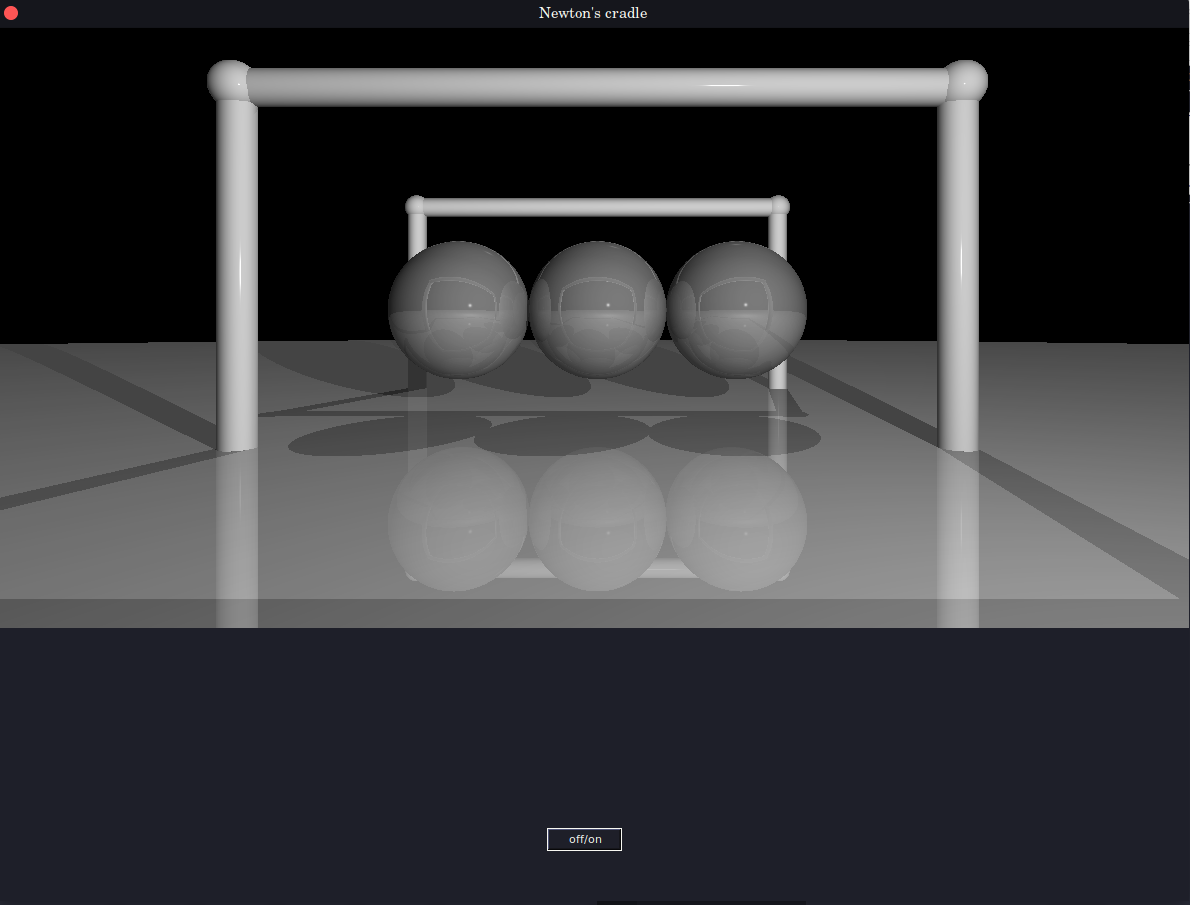
\includegraphics[width=1\textwidth]{res1.png}
		\caption{Результат работы программы 1}
		\label{ref:res1}}
\end{figure}

\begin{figure}[ht!]
	\centering{
		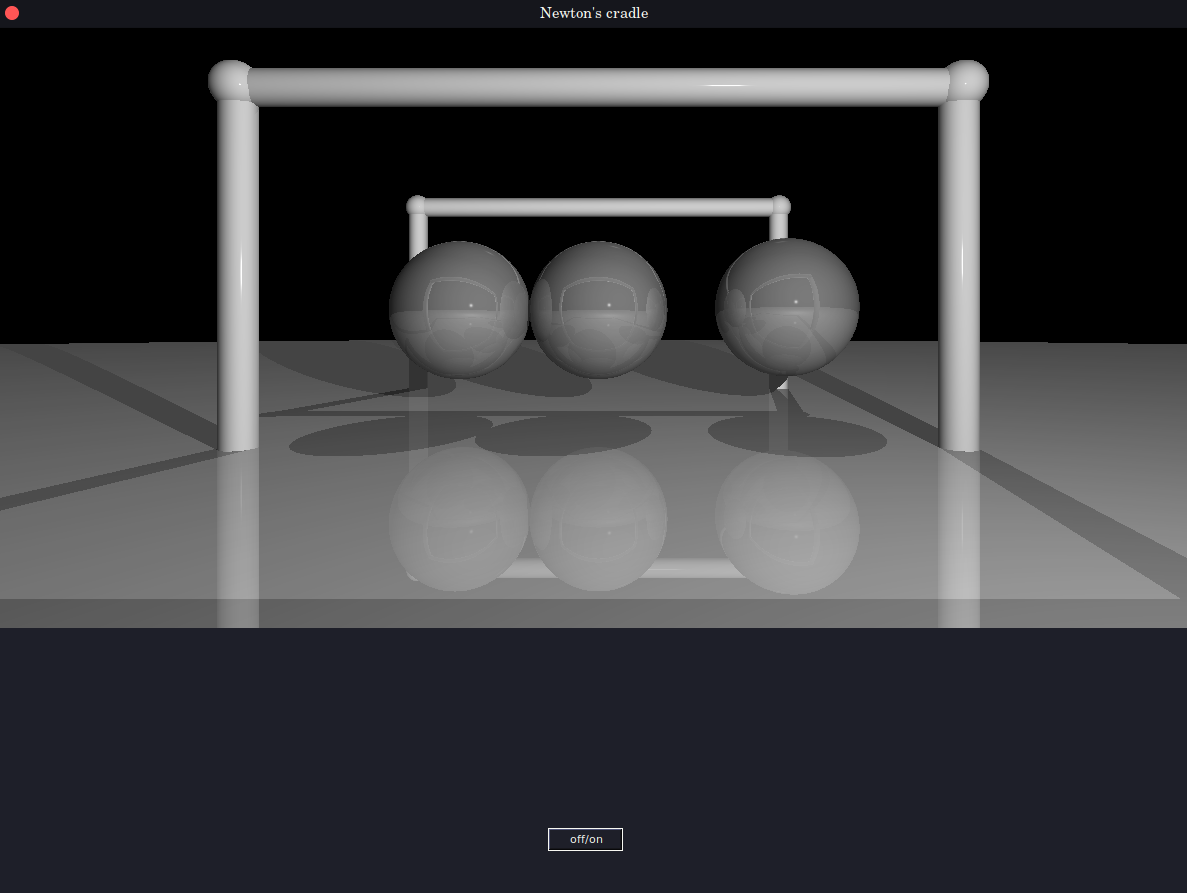
\includegraphics[width=1\textwidth]{res2.png}
		\caption{Результат работы программы 2}
		\label{ref:res2}}
\end{figure}

\section{Вывод}

В данном разделе было произведено сравнение алгоритма трассировки лучей
при простой реализации и многопоточной (рис. \ref{ref:time}).
Результат показал, что выгоднее всего использовать все ядра процессора.
Так же была продемонстрирована работа программы (рис. \ref{ref:res1} и \ref{ref:res2}).